% !TEX encoding = UTF-8
% !TEX TS-program = pdflatex
% !TEX root = ../tesi.tex

\chapter{ROFF}
\label{chapter:roff}

RObust and Fast Forwarding scheme (ROFF) is a protocol proposed by Hongseok Yoo and Dongkyun Kim in \cite{6906275}. This chapter will present the two main problems tackled by ROFF already introduced in Section \ref{sec:emd}, namely the perfect suppression of redundant transmissions, which will be explained in \ref{ssec:collision-analysis} , and the disuniformity and the costant change in spatial vehicle distribution in VANETs, addressed in section \ref{ssec:latency-analysis}.

	\section{Forwarder Selection Problem}
		\subsection{Collision Analysis}
		\label{ssec:collision-analysis}
		The first problem tackled by ROFF concerns collisions caused by nodes who start to transmit at the same time. This results in a collision in the area resulting from the intersection of the nodes' transmission ranges.
		
		
		Suppose that $S_f=\{f_i | 0 < i \leq N, i \in \mathbb{N} \}$ is the set of PFCs ordered in ascending order by the distance between the previous forwarder and the PFC, where N is the number of PFCs and $f_n$ is the FFC. We define $f_0$ as the previous forwarder.
%		TODO immagine con 1..n PFC
		Based on the most common idea in existing protocols, ideally a PFC $f_i$ suppresses its scheduled transmission whenever it receives the transmission from $f_N$. In order to achieve suppression, vehicles from $f_i$ to $f_i-1$ should wait until they receive the transmission from $f_N$ before forwarding. If a vehicle forwards the message before having received the transmission from $f_N$, then a collision will occur. As stated in Section \ref{sec:emd}, existing protocols employ a strategy for waiting time assignment by which each PFC calculates its waiting time based on the distance between itself and the previous forwarder (that is $distance = d(f_i, f_0)$). As a consequence, successful suppression of all PFCs ($f_1$ to $f_{N-1}$, $f_{N-1}$ included) can be achieved only if the timer of $f_{N-1}$ is long enough to detect the transmission from $f_N$. The authors define $minDiff$ as the minimum time difference between $f_N$ and $f_{N-1}$ to prevent $f_{N-1}$ from forwarding.
		
		\begin{figure}[H]
			\centering
			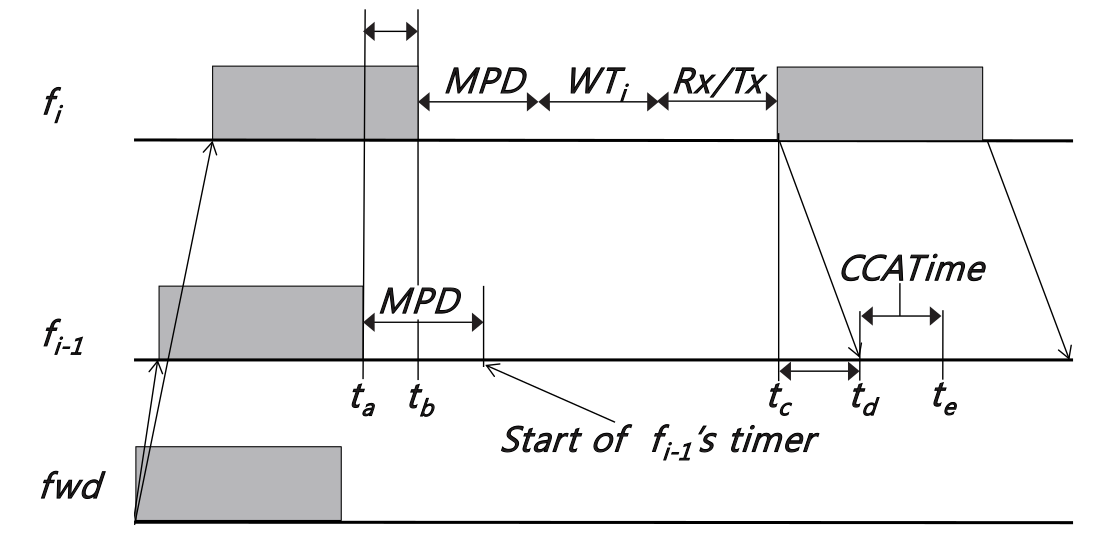
\includegraphics[width=\textwidth]{immagini/minDiff}
			\caption{Definition of $minDiff$ between $f_N$ and $f_{N-1}$ (\cite{6906275})}
			\label{fig:minDiff}
		\end{figure}
	
		\imgrefcap{fig:minDiff} depicts a situation where $fwd$ is the forwarder and $f_i$ (farther from fwd than $f_{i-1}$) relays the message before $f_{i-1}$. The two vehicles $f_i$ and $f_{i-1}$ complete receiving the message at different times ($t_a$ and $t_b$) due to propagation delay (calculated as $propagationDelay = d / s$, where $d$ is the distance between two points in space and $s$ is the wave propagation speed of the medium, i.e. $s=c$, the speed of light, in wireless communication). After reception we have additional amount of time in order to process and retransmit the message:
		\begin{itemize}
			content...
		\end{itemize}
		
		
		
		
		\subsection{Latency Analysis}
		\label{ssec:latency-analysis}